\section{Programmation Orientée Objet \emph{(POO)}}

\begingroup
\setbeamercolor{background canvas}{bg=foreground}
\begin{frame}
    \begin{center}
        \vspace{1cm}
        {\Large Programmation Orientée Objet \emph{(POO)}}
    \end{center}
\end{frame}
\endgroup

\begin{frame}[fragile]
  \begin{columns}[c]
    \column{2.3in}
    \begin{center}{\large Field (champ)}\end{center}
    \begin{csharpcode*}{fontsize=\scriptsize}
public class Circle
{
    public double radius;
    public string color;
}
    \end{csharpcode*}
    \pause
    \begin{center}{\large Method}\end{center}
    \begin{csharpcode*}{fontsize=\scriptsize}
public class Circle
{
    public double radius;
    public string color;

    public void setColor(string newColor)
    {
      this.color = newColor;
    }
}
    \end{csharpcode*}
    \pause
    \column{2.2in}
    \begin{center}
      {\large Property (propriété)}\\
      \emph{\scriptsize Snippet VS : propfull}
    \end{center}
    \begin{csharpcode*}{fontsize=\scriptsize}
public class Truc
{
    // backing field
    private int _attribut;

    public int Attribut // propriété
    {
        get { return _attribut; }
        set { _attribut = value; }
    }
}
    \end{csharpcode*}
  \end{columns}
\end{frame}

\begin{frame}[fragile]
    \begin{center}{\large Validation}\end{center}
    \begin{csharpcode*}{fontsize=\scriptsize}
class Thermostat
{
    private int _temperature; // backing field

    public int Temperature // propriété
    {
        get { return _temperature; }
        set
        {
            if (value >= 50)
                _temperature = 50;
            else
                _temperature = value;
        }
    }
}
    \end{csharpcode*}
\end{frame}

\begin{frame}[fragile]
    \begin{center}
        {\large Auto-propriété}\\
        \emph{\scriptsize Snippet VS : prop}
    \end{center}
    \begin{csharpcode}
public class Objet
{
    public int Attribut { get; set; };
}
    \end{csharpcode}
    \pause
    \begin{center}
        {\large Accès privé sur le \emph{set}}\\
        \emph{\scriptsize Snippet VS : propg}
    \end{center}
    \begin{csharpcode}
public class Objet
{
    public int Attribut { get; private set; };
}
    \end{csharpcode}
\end{frame}

\begin{frame}[fragile]
    \begin{center}{\large Interface}\end{center}
    \begin{csharpcode*}{fontsize=\scriptsize}
interface IBicycle
{
     string BrandName { get; set; }

     void ChangeSpeed(int newValue);

     void Brake();
}
    \end{csharpcode*}
    \pause
    \begin{csharpcode*}{fontsize=\scriptsize}
class BlueBicycle : IBicycle
{
    private string _brandName;

    public string BrandName
    {
        get { return _brandName; }
        set { _brandName = lowerCase(value); }
    }
}
    \end{csharpcode*}
\end{frame}

\begingroup
\setbeamercolor{background canvas}{bg=foreground}
\begin{frame}
  \begin{center}
      \vspace{1.1cm}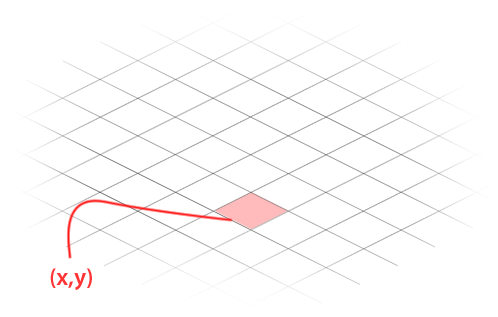
\includegraphics[scale=0.4]{img/map.png}
  \end{center}
\end{frame}

\begin{frame}
  \begin{center}
      \vspace{1.1cm}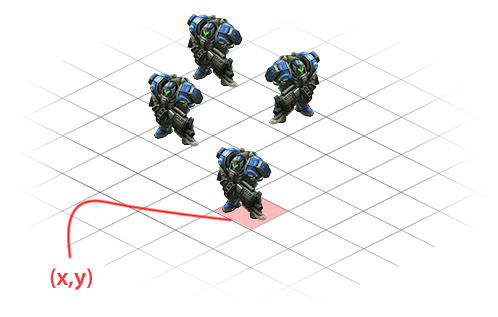
\includegraphics[scale=0.4]{img/unit.png}
  \end{center}
\end{frame}
\endgroup

\begin{frame}[fragile]
\begin{center}{\large Modélisation d'une unité}\end{center}
  \begin{csharpcode*}{fontsize=\scriptsize}
class Unit
{
    public Tuple<int,int> Position { get; set; }

    public int HealthPoints { get; set; }
    private int _maxHealthPoints;

    public int Speed { get; private set; }

    public int Dps { get; private set; }

    public void Move(Tuple<int,int> destination)
    {
        // Bouger
    }

    public void Die()
    {
        // Mourir
    }
}
  \end{csharpcode*}
\end{frame}

\begingroup
\setbeamercolor{background canvas}{bg=foreground}
\begin{frame}
  \begin{center}
    \vspace{1.4cm}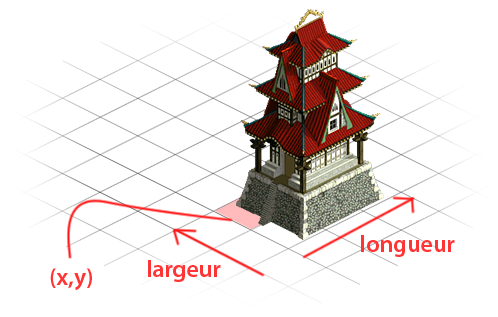
\includegraphics[scale=0.4]{img/building.png}
  \end{center}
\end{frame}
\endgroup


\begin{frame}[fragile]
\begin{center}{\large Modélisation d'un bâtiment}\end{center}
        \begin{csharpcode*}{fontsize=\scriptsize}
class Building
{
    public Tuple<int,int> Position { get; private set; }
    public Tuple<int,int> Size { get; private set; }

    public List<Unit> Units { get; set; }

    public int HealthPoints { get; set; }
    private int _maxHealthPoints;

    public void Die()
    {
        // Mourir
    }
}
        \end{csharpcode*}
\end{frame}

\begin{frame}[fragile]
  \begin{columns}[c]
    \column{2.3in}
    \begin{csharpcode*}{fontsize=\tiny}
class Unit
{
    public Tuple<int,int> Position { get; set; }

    public int HealthPoints { get; set; }
    private int _maxHealthPoints;

    public int Speed { get; private set; }

    public int Dps { get; private set; }

    public void Move(Tuple<int,int> destination)
    {
        // Bouger
    }

    public void Die()
    {
        // Mourir
    }
}
    \end{csharpcode*}
    \column{2.5in}
    \begin{csharpcode*}{fontsize=\tiny}
class Building
{
    public Tuple<int,int> Position { get; private set; }
    public Tuple<int,int> Size { get; private set; }

    public List<Unit> Units { get; set; }

    public int HealthPoints { get; set; }
    private int _maxHealthPoints;

    public void Die()
    {
        // Mourir
    }
}
    \end{csharpcode*}
  \end{columns}
\end{frame}

\begin{frame}[fragile]
    \begin{columns}[c]
        \column{2.3in}
        %\begin{center}{\large Classe Abstraite}\end{center}
        \begin{csharpcode*}{fontsize=\scriptsize}
abstract class GameItem
{
    public Tuple<int,int> Position
        { get; private set; }

    public int HealthPoints
        { get; set; }

    private int _maxHealthPoints;

    public abstract void Die();
}
        \end{csharpcode*}
        \pause
        \begin{csharpcode*}{fontsize=\scriptsize}
class Building : GameItem
{
    public Tuple<int,int> Size
        { get; private set; }

    public List<Unit> Units
        { get; set; }

    public override void Die()
    {
        // Mourir
    }
}
        \end{csharpcode*}
        \column{2.3in}
        \pause
        \begin{csharpcode*}{fontsize=\scriptsize}
class Unit : GameItem
{
    public int Speed
        { get; private set; }

    public int Dps
        { get; private set; }

    public void Move(
        Tuple<int,int> destination)
    {
        // Bouger
    }

    public override void Die()
    {
        // Mourir
    }
}
        \end{csharpcode*}
        \pause
        \begin{center}{\large Héritage}\end{center}
    \end{columns}
\end{frame}

\begin{frame}[fragile]
  \begin{csharpcode*}{fontsize=\scriptsize}
class MyClass
{
    public void MyFonction()
    {
        List<GameItem> gameItems = new List<GameItem>();

        gameItems.Add(new Unit());
        gameItems.Add(new Building());
    }
}
    \end{csharpcode*}
\end{frame}

\begin{frame}[fragile]
\begin{center}{\large Virtual methods}\end{center}
  \begin{csharpcode*}{fontsize=\scriptsize}
abstract class Unit
{
    public virtual void Die()
    {
        // A single death is a tragedy; a million deaths is a statistic.
    }
}
  \end{csharpcode*}
  \pause
  \begin{csharpcode*}{fontsize=\scriptsize}
class Bomber : Unit
{
    public override void Die()
    {
        // Kill everyone around before actually dying

        base.Fonction(parameter);
    }
}
    \end{csharpcode*}
\end{frame}
